\chapter{Evaluación histórica (1980–2014)}\label{cap:4}

\section{Evaluación histórica (1980--2014)}\label{sec:eval}

Esta sección responde la primera pregunta del estudio: una vez igualada la frecuencia de días húmedos (criterio i; R₀ = 5,285 mm día$^{-1}$ en ALADIN y R = 1 mm día$^{-1}$ en CR2MET), ¿reproduce ALADIN la distribución histórica de duraciones de dry spells?

\subsection{Climatología de persistencia en CR2MET}\label{sec:climatologia}

CR2MET muestra un contraste norte--sur marcado en la persistencia de rachas secas, coherente con el gradiente climático de Chile y con diagnósticos recientes de dry spells en la zona central (Latoja et al., 2025; Herrera-Marín et al., 2026). En el norte árido la duración media supera con creces el mes: en la ventana del Loa el pool regional tiene media de 65,6 días y p99 de 456 días, con máximos por encima de 1 400 días. En el sur más húmedo las rachas son cortas y numerosas: en Biobío la media es 6,2 días y el p99, 44 días. Maipo y Maule ocupan el tramo intermedio (medias de 11,0 y 9,5 días; p99 de 119 y 83 días). Ese gradiente no es un artefacto de un índice anual: aparece tanto en la media como en la cola (t99) a escala de píxel (Figura~\ref{fig:mapas}, columnas CR2MET).

Dos implicaciones siguen de inmediato. Primera: un mismo estadístico agregado ---por ejemplo, el CDD--- comprime climas distintos en un solo máximo por año (Zhang et al., 2011; Sillmann et al., 2013a), mientras que aquí la cola de Loa y la de Biobío no son conmensurables. Segunda: cualquier evaluación de ALADIN tiene que respetar ese contraste latitudinal; un sesgo aceptable en el sur húmedo puede ser grave en el desierto si se pierde la cola de spells de cientos de días.

\subsection{ALADIN reproduce el gradiente espacial, pero subestima la persistencia y la cola}\label{sec:sesgo}

Con el criterio i, ALADIN reproduce el patrón espacial ---norte persistente, sur de rachas cortas--- pero subestima la duración. Sobre Chile continental, la duración media espacial es 42,1 días en CR2MET y 34,0 días en ALADIN (Δ, media espacial de las diferencias por píxel, = −8,2 días). El sesgo es mayor en la cola: t99 espacial de 221,1 días frente a 175,3 días (Δ = −46,3 días). Los mapas de diferencia (Figura~\ref{fig:mapas}) muestran Δ negativo de manera generalizada, más intenso en la transición norte--centro, donde CR2MET resuelve spells extremadamente largos que ALADIN acorta. ALADIN es significativamente más corto en cerca de dos tercios de los píxeles para la duración media (65 \%) y en el 43 \% para t99 (bootstrap por años, IC95 de Δ que no incluye cero).

Ese residuo no se explica solo por el umbral. Con 1 mm en ambos productos (criterio ii) el sesgo aumenta mucho (Δ media ≈ −27 días; Δ t99 ≈ −135 días). El R₀ global (criterio i) lo reduce sustancialmente; a escala nacional, el R₀ local lo reduce algo más, pero no elimina el sesgo de cola (Tabla~\ref{tab:S1}; Figura~\ref{fig:S1}). El análisis principal usa el criterio i porque corrige la definición de día húmedo sin un campo heterogéneo de umbrales; el sesgo residual se interpreta como limitación del RCM.

\begin{figure}[htbp]
\centering
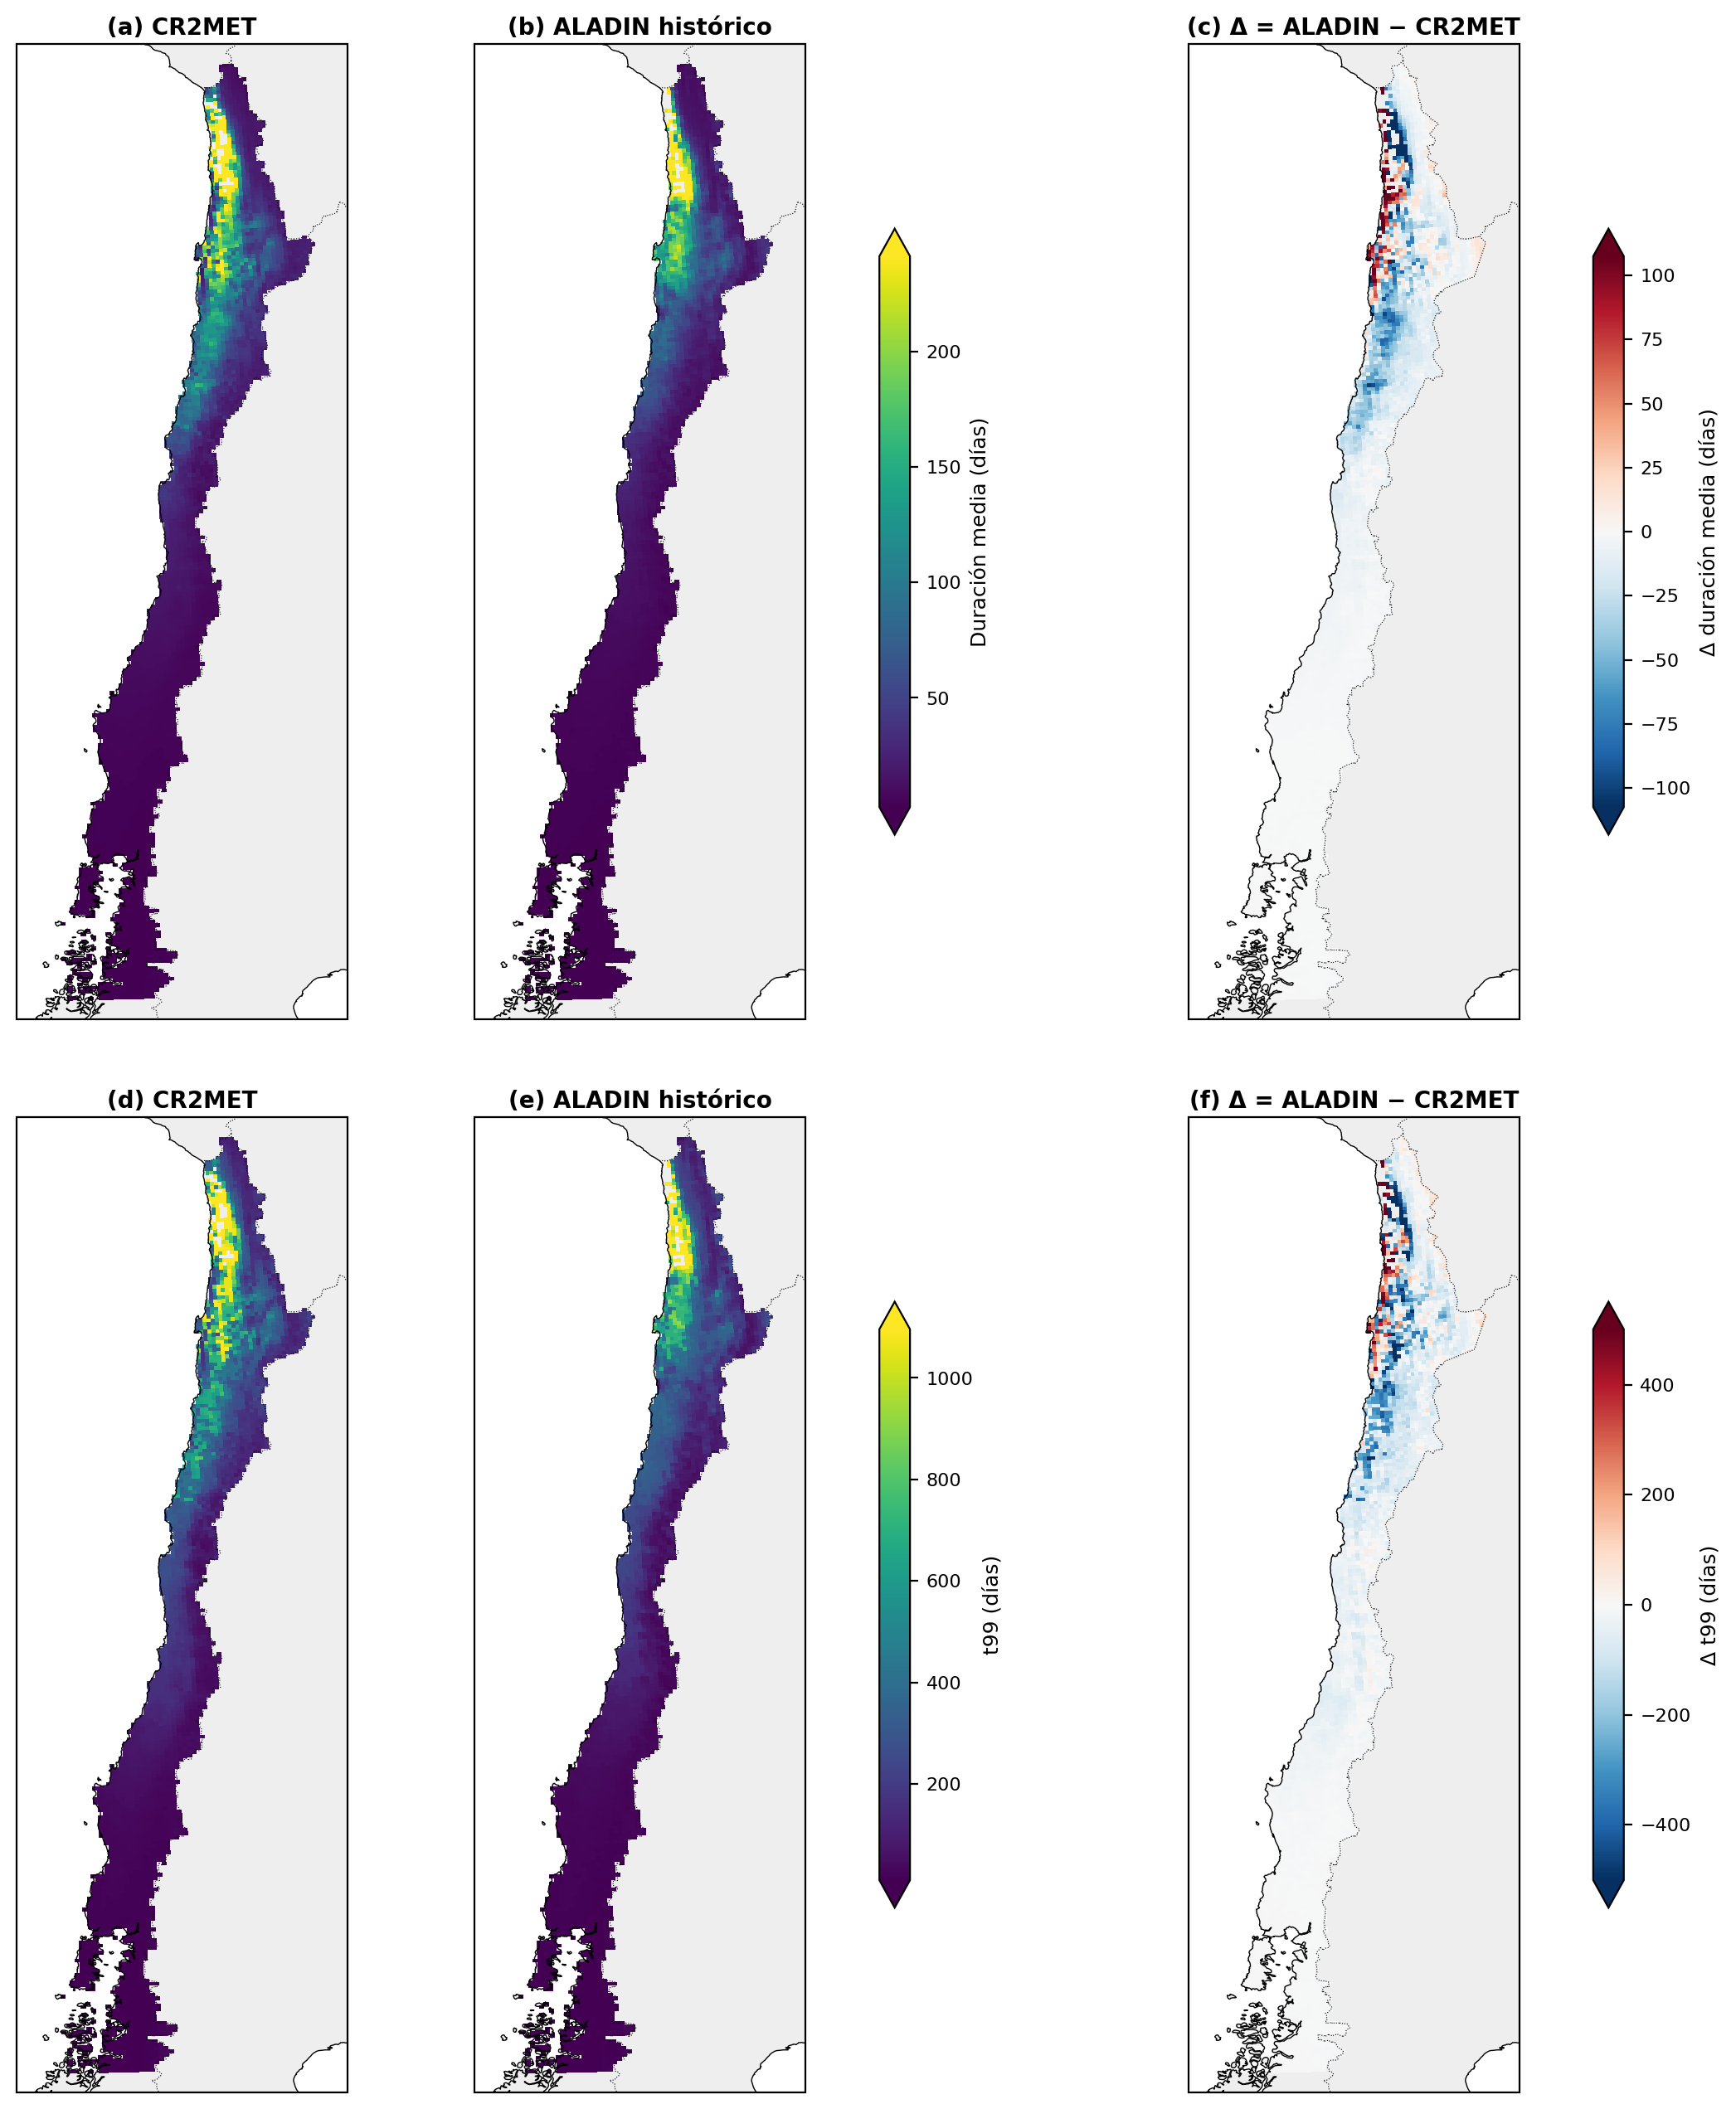
\includegraphics[width=1\linewidth,height=0.72\textheight,keepaspectratio,alt={Persistencia histórica de dry spells (1980--2014), criterio i. Fila superior: duración media (días). Fila inferior: percentil 99 de las duraciones, t99 (días). Columnas: CR2MET regrillado (R = 1 mm), ALADIN histórico (R₀ = 5,285 mm) y Δ = ALADIN − CR2MET. Ambas fuentes reproducen el gradiente norte--sur; ALADIN subestima media y cola, con Δ negativo más marcado en t99.}]{fig32_persistencia_spatial_only.png}
\caption[Persistencia histórica de dry spells (1980--2014), criterio i]{Persistencia histórica de dry spells (1980--2014), criterio i. Fila superior: duración media (días). Fila inferior: percentil 99 de las duraciones, t99 (días). Columnas: CR2MET regrillado (R = 1 mm), ALADIN histórico (R₀ = 5,285 mm) y Δ = ALADIN − CR2MET. Ambas fuentes reproducen el gradiente norte--sur; ALADIN subestima media y cola, con Δ negativo más marcado en t99.}\label{fig:mapas}
\end{figure}

\subsection{PDFs regionales: buen acuerdo en el centro-sur y mayor sesgo de cola en el norte}\label{sec:pdfs_hist}

Las distribuciones regionales confirman que el acuerdo entre CR2MET y ALADIN es mayor en el centro-sur y que el principal desacuerdo se concentra en la cola del norte árido (Figura~\ref{fig:pdfs}; Tabla~\ref{tab:estadisticos}). En Maipo, Maule y Biobío, CR2MET e histórico de ALADIN son aproximadamente paralelos: ALADIN captura la forma y subestima de manera moderada las duraciones (medias 8,6 frente a 11,0 días en Maipo; 7,3 frente a 9,5 en Maule; 5,3 frente a 6,2 en Biobío). En Loa el desacuerdo se concentra en la cola: CR2MET mantiene más probabilidad en spells de cientos de días (p99 = 456 días frente a 360 días en ALADIN; máximo 1 419 frente a 1 156). ALADIN produce, en todas las cuencas, más spells que CR2MET (p.~ej. 66 267 frente a 55 015 en Loa), coherente con rachas algo más cortas aunque la frecuencia de wet days ya está emparejada.

En conjunto, la evaluación histórica muestra que ALADIN reproduce mejor la forma de la distribución en Maipo, Maule y Biobío, mientras que subestima las duraciones en el norte árido y en la cola extrema.

\begin{longtable}[]{@{}llllllll@{}}
\caption[Estadísticos del pool regional de duraciones de dry spells (criterio i; 1980--2014 y 2040--2074)]{Estadísticos del pool regional de duraciones de dry spells (criterio i; 1980--2014 y 2040--2074). n\_spells es el número de rachas en el pool; p90 y p99 están en días.}\label{tab:estadisticos}\tabularnewline
\toprule\noalign{}
Cuenca & Producto & n\_spells & Media & Mediana & p90 & p99 & Máx. \\
\midrule\noalign{}
\endfirsthead
\toprule\noalign{}
Cuenca & Producto & n\_spells & Media & Mediana & p90 & p99 & Máx. \\
\midrule\noalign{}
\endhead
\bottomrule\noalign{}
\endlastfoot
Loa & CR2MET hist & 55 015 & 65,6 & 23 & 185 & 456 & 1 419 \\
Loa & ALADIN hist & 66 267 & 54,6 & 22 & 143 & 360 & 1 156 \\
Loa & ALADIN fut & 64 043 & 56,6 & 25 & 151 & 385 & 1 853 \\
Maipo & CR2MET hist & 150 209 & 11,0 & 5 & 23 & 119 & 283 \\
Maipo & ALADIN hist & 181 049 & 8,6 & 4 & 18 & 87 & 194 \\
Maipo & ALADIN fut & 159 887 & 10,0 & 4 & 21 & 112 & 224 \\
Maule & CR2MET hist & 184 462 & 9,5 & 5 & 21 & 83 & 206 \\
Maule & ALADIN hist & 228 077 & 7,3 & 4 & 17 & 57 & 160 \\
Maule & ALADIN fut & 202 463 & 8,6 & 4 & 19 & 76 & 188 \\
Biobío & CR2MET hist & 344 251 & 6,2 & 4 & 14 & 44 & 109 \\
Biobío & ALADIN hist & 399 130 & 5,3 & 3 & 12 & 34 & 153 \\
Biobío & ALADIN fut & 370 260 & 6,0 & 3 & 14 & 39 & 120 \\
\end{longtable}

\begin{figure}[htbp]
\centering
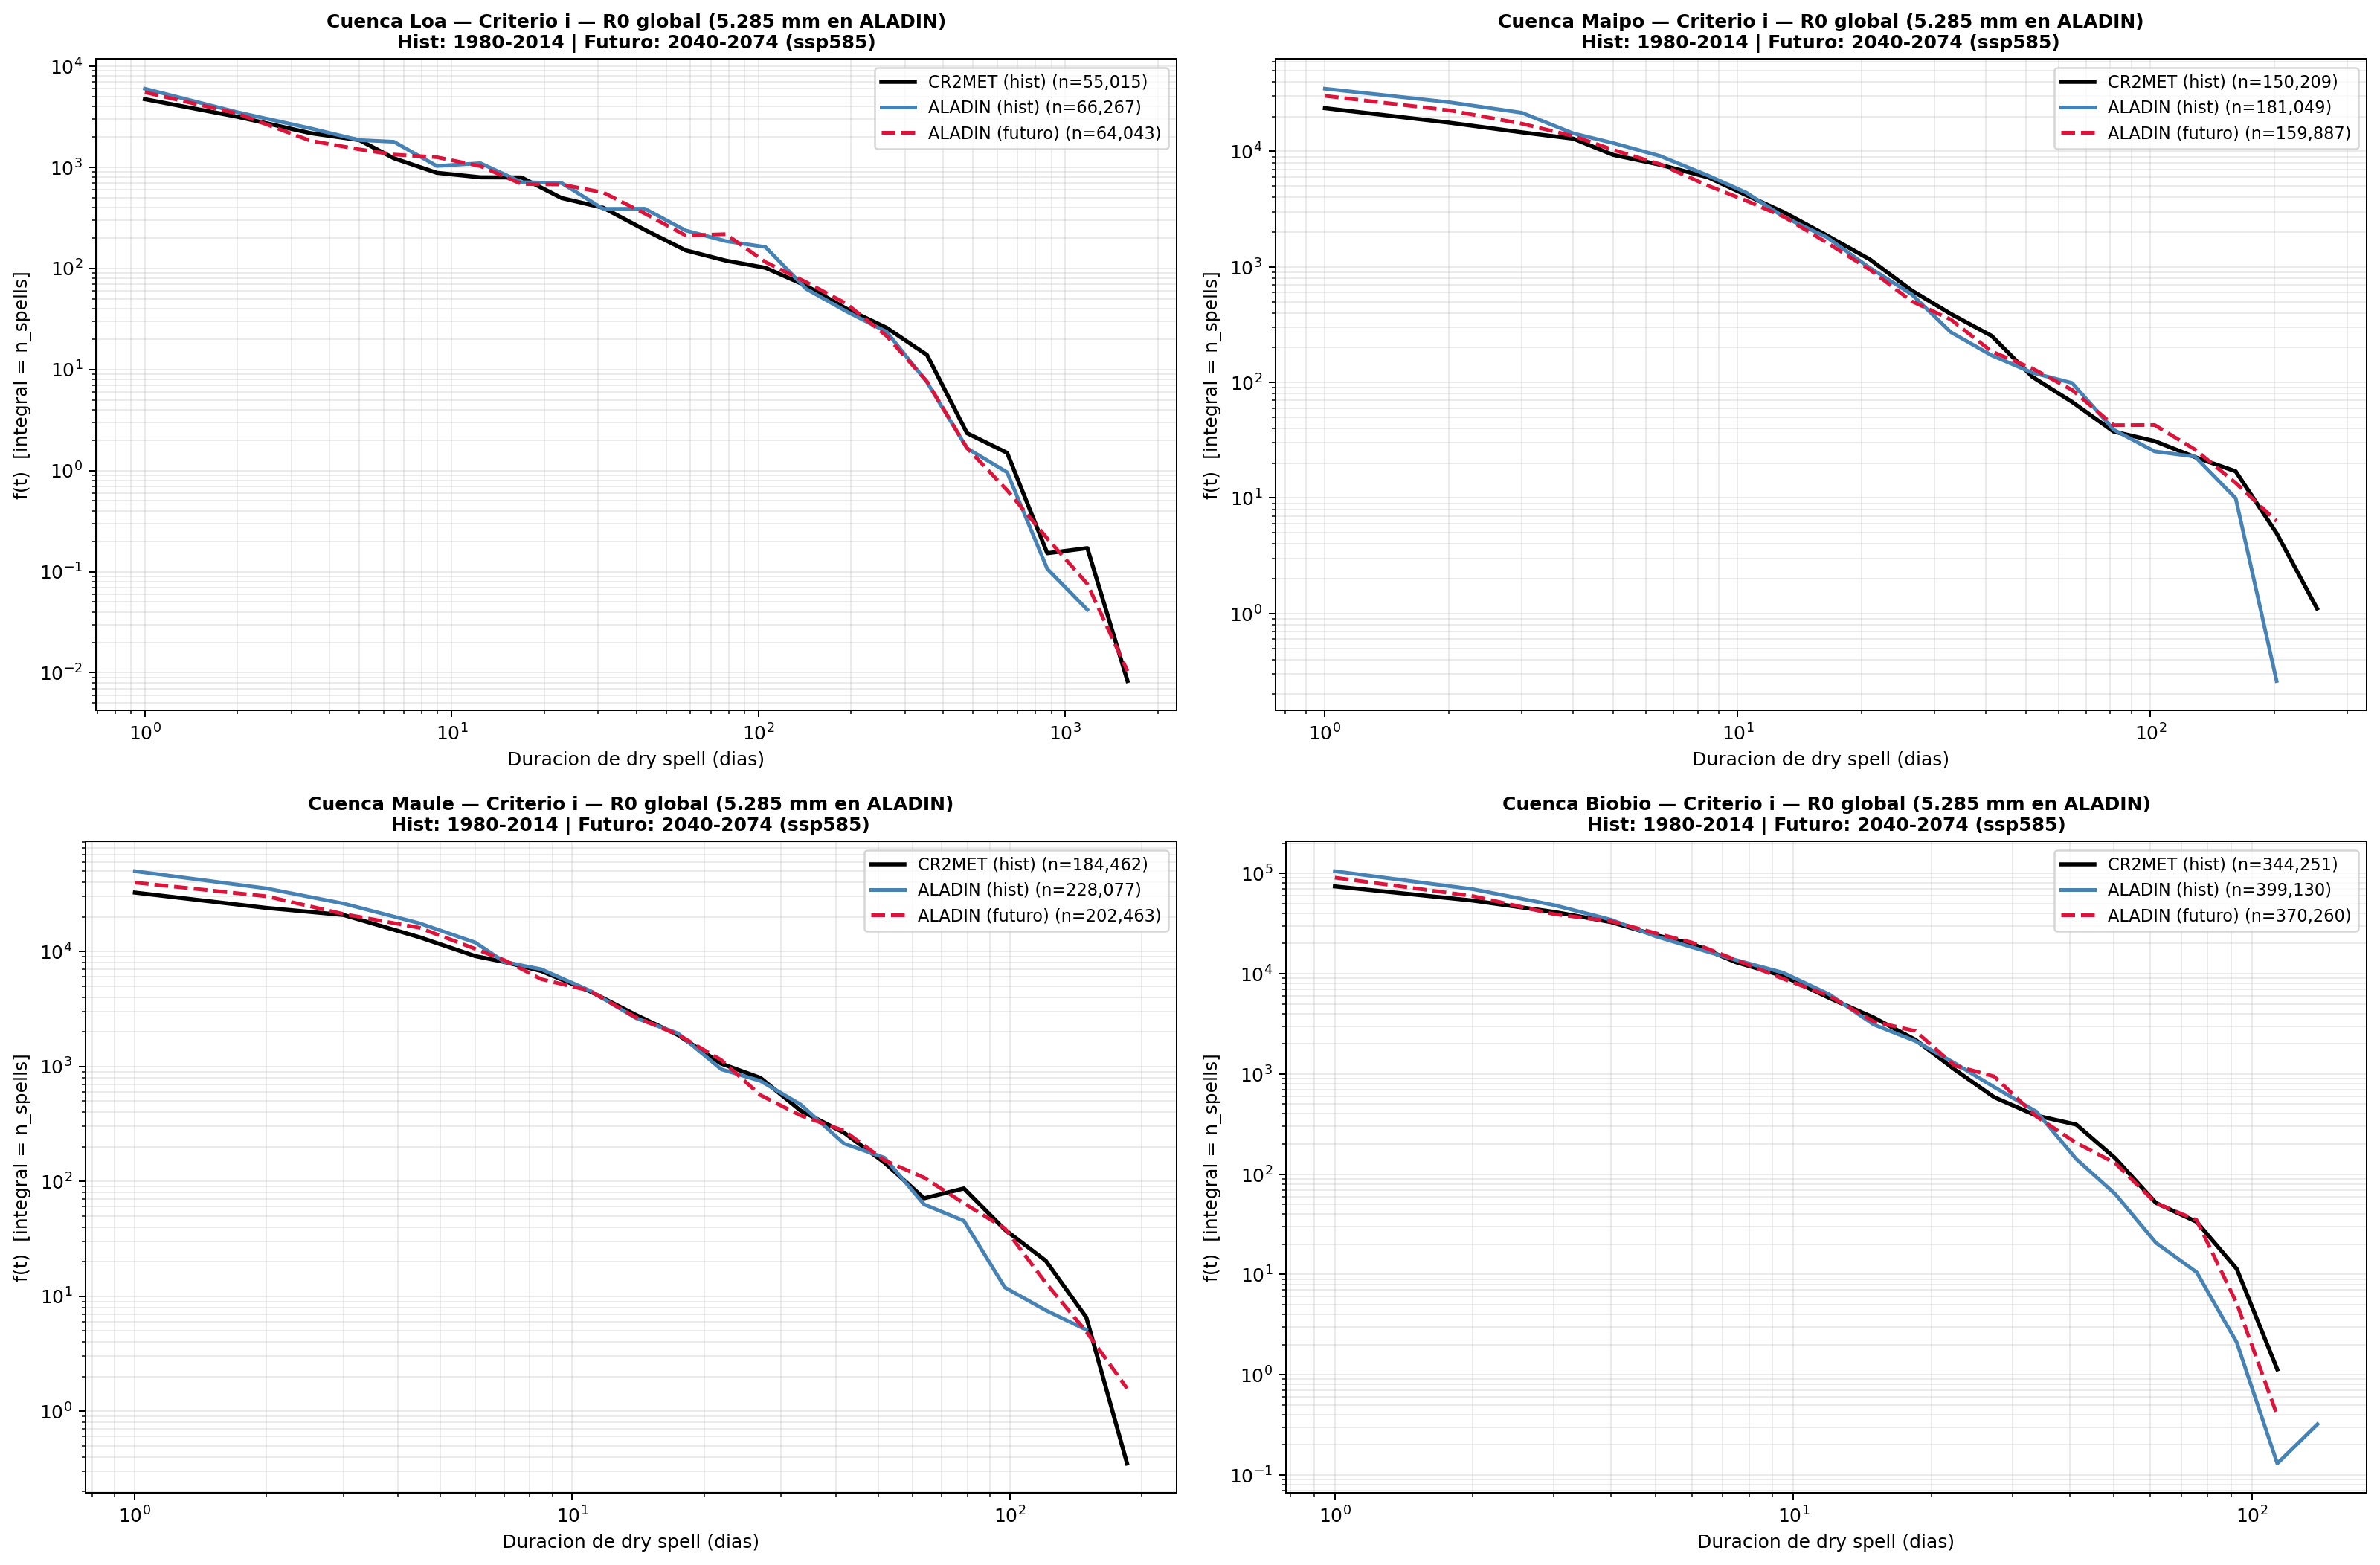
\includegraphics[width=1\linewidth,height=0.72\textheight,keepaspectratio,alt={PDFs empíricas de duración de dry spells (criterio i, escala log--log; ∫ f dt = n\_spells). Negro: CR2MET 1980--2014. Azul: ALADIN histórico. Rojo discontinuo: ALADIN futuro (SSP5-8.5, 2040--2074). El histórico de ALADIN sigue la forma de CR2MET en Maipo, Maule y Biobío, y pierde cola en Loa. El futuro se discute en §\ref{sec:pdfs_fut}: n\_spells disminuye y la cola derecha se extiende en las cuencas centrales y en Biobío.}]{fig42_pdf_cuencas_loglog_panel.png}
\caption[PDFs empíricas de duración de dry spells (criterio i, escala log--log; ∫ f dt = n\_spells)]{PDFs empíricas de duración de dry spells (criterio i, escala log--log; ∫ f dt = n\_spells). Negro: CR2MET 1980--2014. Azul: ALADIN histórico. Rojo discontinuo: ALADIN futuro (SSP5-8.5, 2040--2074). El histórico de ALADIN sigue la forma de CR2MET en Maipo, Maule y Biobío, y pierde cola en Loa. El futuro se discute en §\ref{sec:pdfs_fut}: n\_spells disminuye y la cola derecha se extiende en las cuencas centrales y en Biobío.}\label{fig:pdfs}
\end{figure}

\pendiente{decidir si las sensibilidades S1--S3 y S5 (Anexo A) se integran aquí
como sección de robustez.}
